%vamp.tex
% notes for development of VAMP (Vesicle Aspiration with MicroPipettes) project
% all figures concerning Phase Contrast images are based on image file
% pshchelo\images\pipettes\PhC\me\micropipettes6\ves_-000100.tif = phc-test1.tif

\chapter{Notes for development of image analysis for Vesicle Aspiration with MicroPipettes experiments}\label{chap:devnotes}

The whole project can be divided in three ``subprojects'', which are mostly independent on each other in terms of development, but rather produce an input for next step:
\begin{enumerate}
	\item Experiment automatisation
	\item Data extraction from images
	\item Data analysis
\end{enumerate}
Let's consider these steps more closely

\section{Experiment automatisation - LabVamp}\label{experiment}

Since the project presumes development of software running on 3 different experimental setups, \emph{LabView}\copyright{} environment was chosen for this part. This should enable creating the core of the automation procedure common for all three setups and then just plugging in specific device drivers.

Currently the LabView program (dubbed LabVamp) consist of 3 blocks: pressure reading, image acquisition and stage movement modules. The main conversation between modules is carried out by SNAP signal, that is ordering the camera to make a snapshot

The pressure reading module is totally independent from all others. Inputs are only parameters for initializing (card number, config file, etc), output is a pressure value.

The image acquisition module besides init values and real-time camera control inputs needs also a SNAP input command from stage controllig module, that will save a current image.

The stage movement module needs (besides init parameters) inputs for desired positions and must output current positions plus SNAP signal.

\section{Extraction of data form images - VamPy}\label{data}

For now everything is done in Python with different additional packages.

It can be considered as a prototype for future C/C++ program, but I really suspect that I will leave it in Python with probably some subroutines rewritten in C/C++ to boost performance --- sticking to Python will definitely shorten development time. Also there exists a \emph{LabPython} package for LabView that allows calling Python from within LabView, which could come in handy when gluing first and second steps.

The pseudocode-like draft for the algorithm for processing single image should look like this:
\begin{enumerate}
  \item get user input
  \item load picture to array
  \item calculate positions of pipette walls
  \item calculate pipette radius
  \item calculate the middle line (axis) of the system
  \item extract data along the axis from the picture
  \item find positions of 3 characteristic points on the axis
  \item calculate all derived parameters (vesicle radius, tip length, surface area, volume)
  \item output these data
\end{enumerate}

Python packages aside from Python Standard Library used or (probably) going to be used in this program:
\begin{itemize}
	\item \emph{numpy} --- basic package for numeric stuff, defines \emph{array} data type
	\item \emph{scipy} --- depends on \emph{numpy} and provides a lot of mathematical functions, which I most probably will need \cite{scipy}
	\item \emph{wxPython} --- GUI programming
	\item \emph{psyco} --- JIT compiler for Python, may use it to speed up the execution
	\item \emph{Python Image Library (PIL)} --- basic image processing functionality, but may eventually drop it (see Section \ref{loadpic})
	\item \emph{matplotlib} --- for plotting results
\end{itemize}

\subsection{Load picture to array}\label{loadpic}

This is done with \emph{scipy} and \emph{PIL}, which allows for direct conversion from image file to \emph{numpy} array.

On the other hand, \emph{wxPython}'s wxImage object could be probably used, thus eliminating the need of \emph{PIL} package, since I'm going to use \emph{wxPython} for GUI programming anyway. Unfortunately, wxImage still doesn't support \emph{numpy}-like array interface as of now, but this is planned feature for addition. Or buffers interface seems to be able to do this \ldots

\subsection{Get user input}\label{getinput}

\begin{figure}
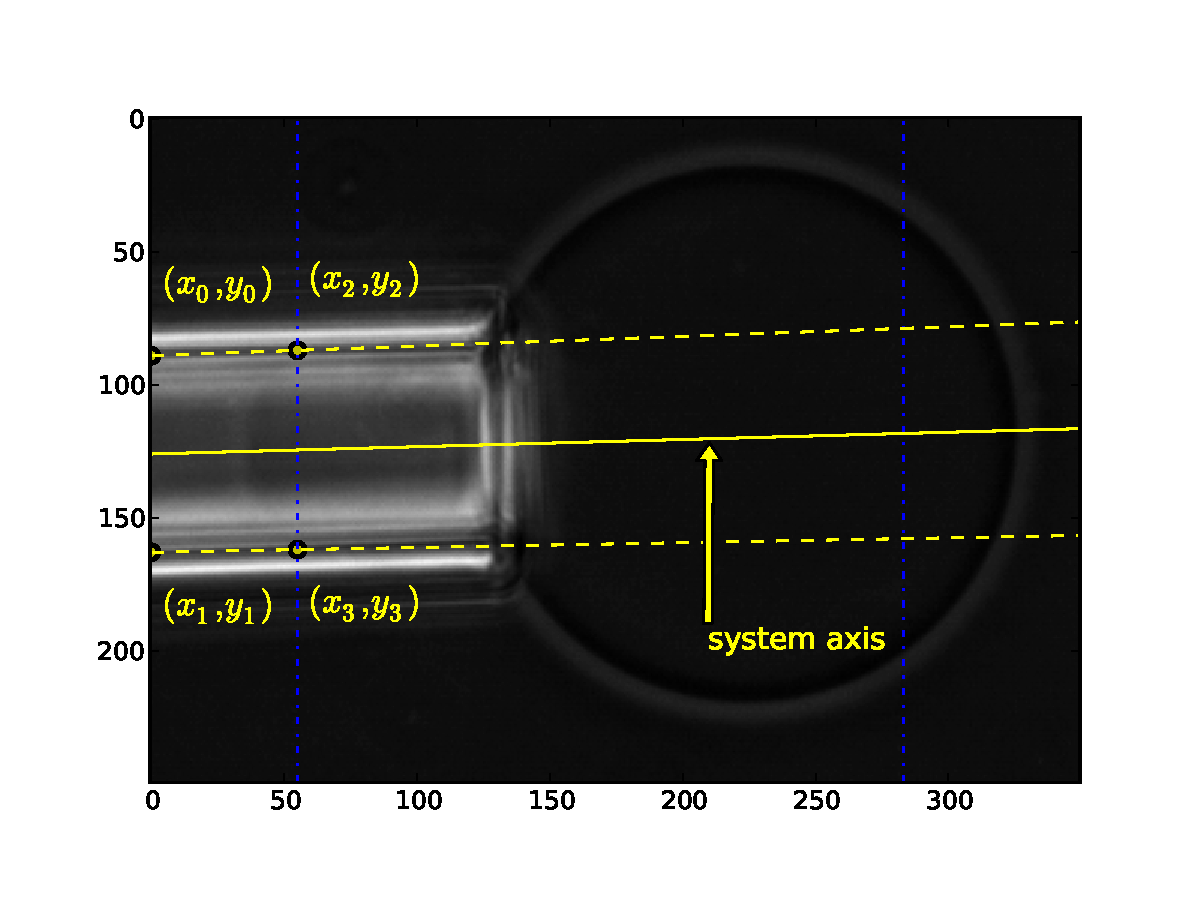
\includegraphics[width=\columnwidth]{figs/pipetteaxis.pdf}
\caption{Sketch of general situation of pipette system alignment on the image}
\label{fig:pipetteaxis}
\end{figure}

First of all user crops the image so that everything but the vesicle is left out and rotates the picture so that the pipette sticks from left.

Now that the orientation of the picture is always the same, user supplies $x$-coordinates of 3 vertical lines - first is just a suitable offset from the left border of the image, second is the overestimated rightmost (closest to the pipette tip) position of the aspirated vesicle tip and the third is the overestimated leftmost (also closest to the pipette tip) position of the outer vesicle edge. (see Fig.~\ref{fig:pipetteaxis}). \textsl{Then the brightness profiles along 1st and 2nd lines are extracted to localize the position of pipette walls. For a phase contrast images inner walls of the pipette are considered to be inner inflection points of sharp minima peaks on the profile (see Fig.~\ref{fig:pipetteprofile}). In order to find them rough positions of the minima are estimated by finding 8 steepest jumps in the second derivative of gaussian-prefiltered (\texttt{scipy.ndimage.gaussian\_laplace()} function) profile across the pipette, with ``2nd and 3rd'' and ``6th and 7th'' defining estimate of peak location. Then the vicinity of estimate position is fitted with Gaussian profiles (for details on fitting procedure see Section~\ref{fitpeak}) and finally corresponding inflection points give sets of coordinates $(x_1,y_1), (x_2,y_2)$ and $(x_3,y_3), (x_4,y_4)$.}

\begin{figure}%
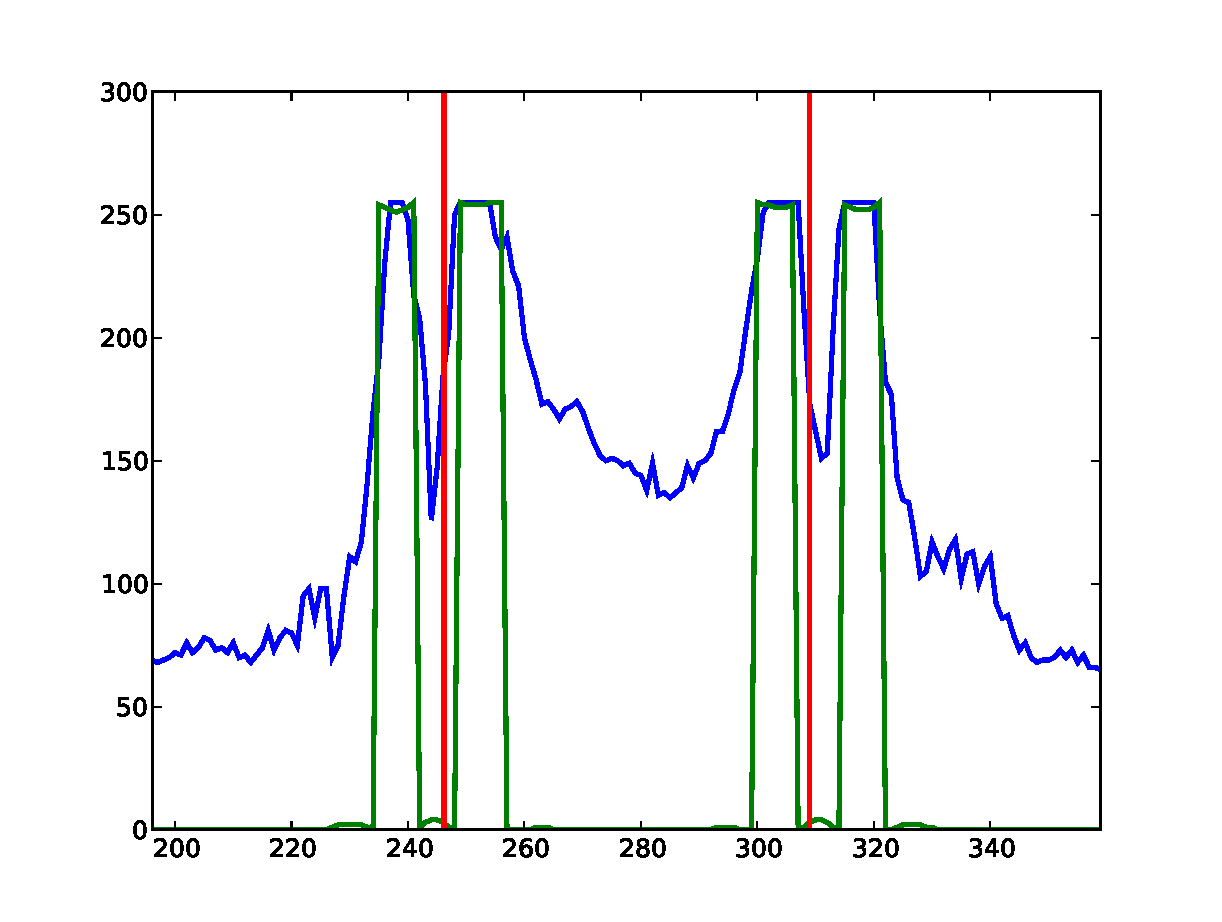
\includegraphics[width=\columnwidth]{figs/pipetteprofile.pdf}%
\caption{Part of brightness profile along the line $(x_1,y_1), (x_2,y_2)$ on Fig.~\ref{fig:pipetteaxis}. Blue line - brightness profile itself, green line - result of applying gaussian-presmoothed laplacian filter, red lines - found positions of inflection points.}%
\label{fig:pipetteprofile}%
\end{figure}

\subsection{Calculate pipette radius}\label{calcpiprad}

Distance (unsigned) from point $\left(x_0,y_0\right)$ to line $y=kx+b$ is given by:
\begin{equation}
\delta = \left|\frac{kx_0+b-y_0}{\sqrt{k^2-1}}\right|\;.
\label{eq:pointtoline}
\end{equation}
Thus the diameter of the pipette for single image is calculated as mean of distances from every of 4 points to the line corresponding to the opposing wall. Then these values are again averaged between all images.

\subsection{Calculate the middle line (axis) of the system}\label{calcaxis}

Having obtained the set of reference points from Section~\ref{getinput} one builds a system axis as a bisector between straight lines formed by pipette inner walls. This is done by simply defying the line going through 2 middle points $\left(\frac{x_1+x_2}{2}, \frac{y_1+y_2}{2}\right)$ and $\left(\frac{x_3+x_4}{2}, \frac{y_3+y_4}{2}\right)$. Then the axis $y = kx+b$ is defined by coefficients

\begin{equation}
k = \frac{y_1+y_1-y_3-y_4}{x_1+x_2-x_3-x_4}, \; b = \frac{y_1+y_2}{2} - k\frac{x_1+x_2}{2}\;\;.
\label{eq:axis}
\end{equation}

After that the brightness profile along this axis is extracted from image with special function (\verb|scipy.ndimage.map-coordinates()|), which returns spline-interpolated values of brightness ``between'' pixels. To define the set of points at which interpolated brightness should be evaluated first intersections of the system axis with boundaries of image are calculated. To define the number of points for evaluation the biggest of differences in $x$ or $y$ coordinates between intersection points is taken.

Small pitfall --- since at the end we need real distances between features, an attention have to be paid to keep the scale of profiles equal. The above procedure does not keep the scale, because the line has only as many points as there are along one of it's coordinates, but it should be $\sqrt{x^2+y^2}$. Hence, the distance between 2 consecutive points on brightness profile along arbitrary tilted straight line with number of evaluated points as defined above corresponds to distance $\epsilon$ in pixels, where
\begin{equation}
\epsilon = \left\{
\begin{array}{ll}
	\sqrt{1+k^2},&\text{if }k < 1\\
	\sqrt{1+\frac{1}{k^2}},&\text{if } k \geq 1 
\end{array}
\right.\;\;,
\label{eq:profilescale}
\end{equation}
so that $1 \leq \epsilon \leq \sqrt{2}$. Thus the procedure of extracting brightness profile must also return the $\epsilon$ value along with profile itself to use it in final steps of determining distances. This is not necessary for profiles used for location of pipette walls, since by design only untilted profiles along pixel lines are used there, thus the scale in preserved.

\subsection{Find positions of 3 characteristic points on the axis}\label{points}

We are interested in 3 points on the axis of the system --- intersection of axis with outer vesicle, aspirated tip of a vesicle and the tip of the pipette. These manifest themselves as peaks (positive or negative) or steep jumps on the brightness profile along the axis. What exactly feature corresponds to what point of interest depends on the type of images one analyses.

\subsubsection{Phase contrast images}\label{phcfeatures}

\begin{figure}%
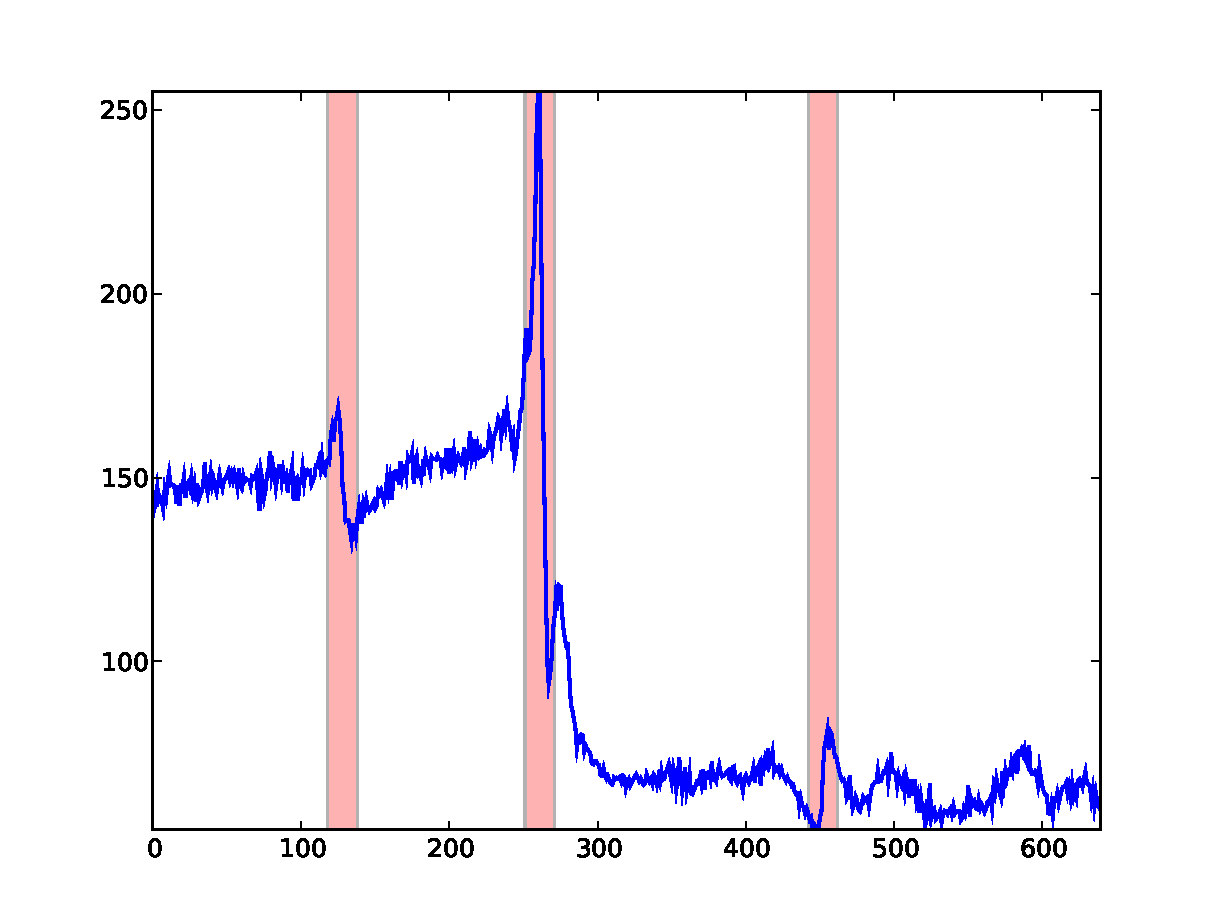
\includegraphics[width=\columnwidth]{figs/phcaxisprofile.pdf}%
\caption{Brightness profile along the system axis for phase contrast image at Fig.~\ref{fig:pipetteaxis}. Red colour denotes approximate regions where features to find are located.}%
\label{fig:phcaxisprofile}%
\end{figure}

For phase contrast images (see Fig.~\ref{fig:phcaxisprofile}), the pipette tip is maximum and vesicle sides are featured as steep jumps from dark to bright (so the inflection point is a choice for a feature position). 

The pipette tip is first roughly located as the global maximum of the whole brightness profile, giving the position of the pipette tip with \emph{pixel resolution}. To get a \emph{subpixel resolution} of peak position we fit it with some suitable profile (see Section \ref{fitpeak}) with parameters of the fit giving the value desired.

The general problem with phase contrast is that the tip of the pipette is so bright and the profile is so smeared, that one can not be strictly sure if the global maximum of the profile corresponds exactly to pipette tip position. But for a time being we will assume that.

As for inflection points, the rough positions are found by first applying \verb|scipy.ndimage.gaussian_gradient_magnitude()| filter (calculates an absolute value of gradient of gaussian-presmoothed profile) and than using user input for overestimated feature positions (see Section~\ref{getinput}) to define left and right search regions where global maxima for these regions are found, giving positions of steep jumps with \emph{pixel resolution} - see Fig.~\ref{fig:phcprofilegrad}. For \emph{subpixel resolution} the profile in the vicinity of estimated position is fitted with suitable function with well-defined inflection point (see Section~\ref{fitjump}).

\begin{figure}%
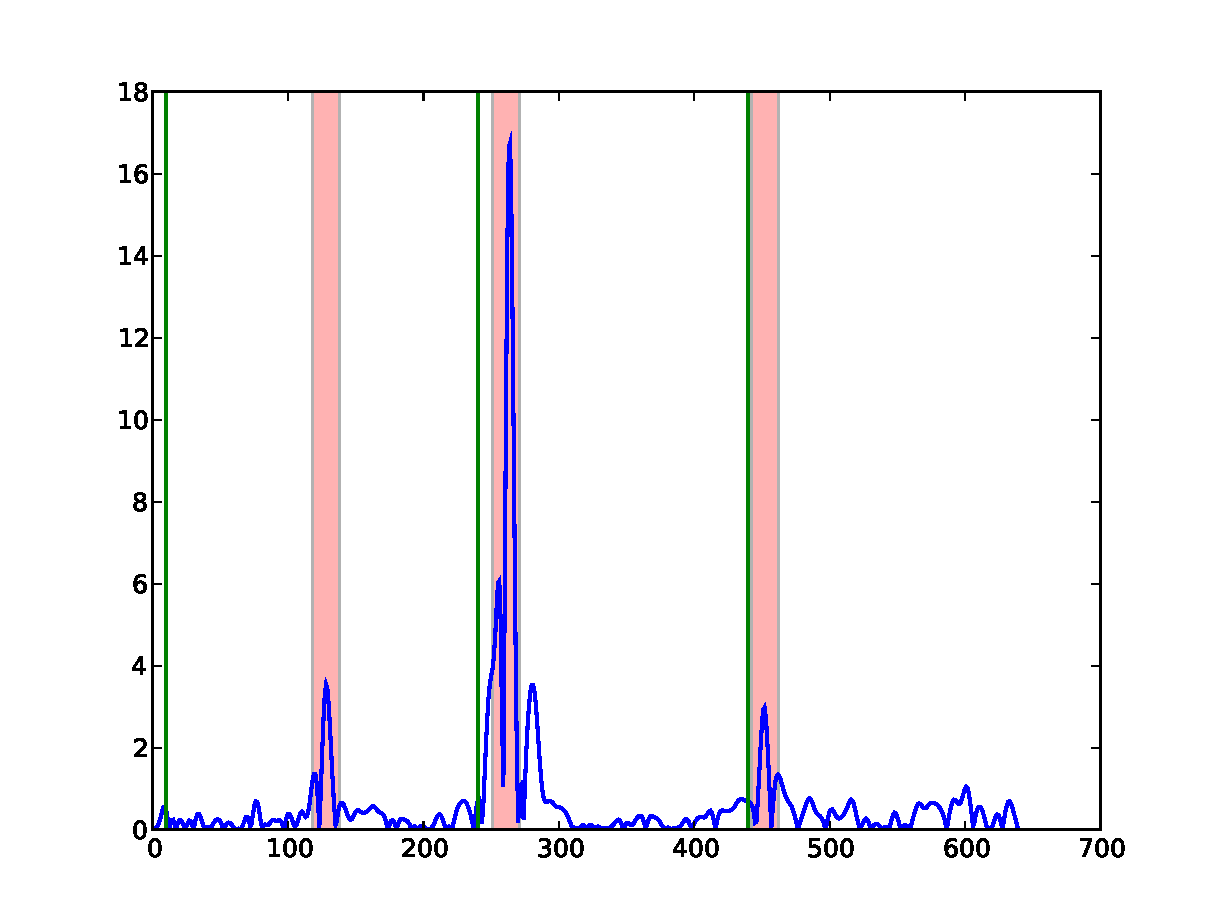
\includegraphics[width=\columnwidth]{figs/phcprofilegrad.pdf}%
\caption{Result of applying gradient magnitude filter to gaussian-presmoothed profile from Fig.~\ref{fig:phcaxisprofile}. Red regions are the same as at Fig.~\ref{fig:phcaxisprofile}. Green lines correspond to user input for overestimated feature positions (see Section~\ref{getinput}).}%
\label{fig:phcprofilegrad}%
\end{figure}

\subsubsection{DIC images}\label{dicfeatures}

For DIC images the inner tip is minimum and the outer edge is maximum (or vise versa, depending on choice of polarizations) and pipette tip is always maximum (see Fig.~\ref{fig:dicaxisprofile}). Problem --- the tip of the pipette creates 2 close peaks, and it not yet completely clear, which of them corresponds exactly to the pipette tip. The fitting procedure by itself is the same as for peaks in~Section~\ref{phcfeatures}.

\begin{figure}%
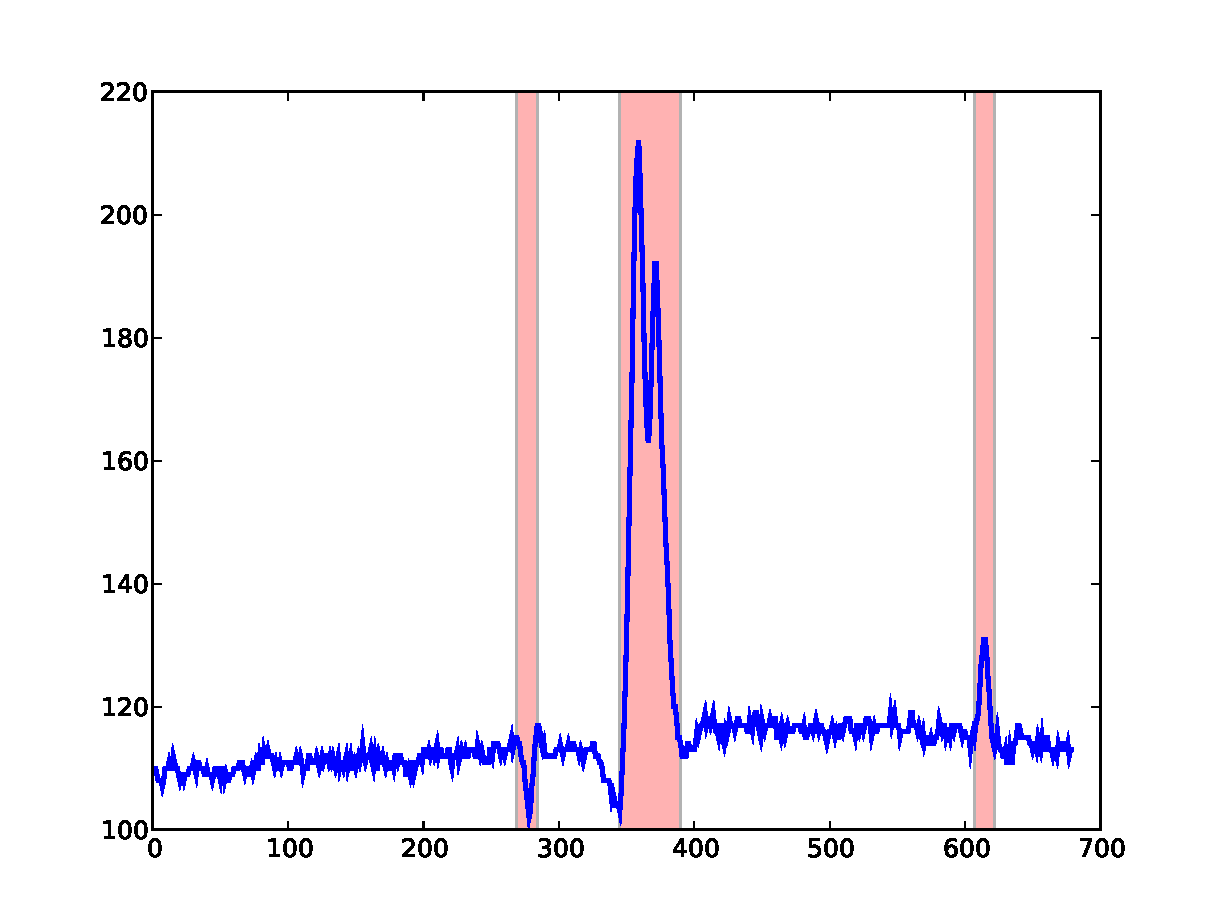
\includegraphics[width=\columnwidth]{figs/dicaxisprofile.pdf}%
\caption{Example of brightness profile along the system axis in DIC image. Red regions denote approximate feature positions.}%
\label{fig:dicaxisprofile}%
\end{figure}

\subsubsection{Fitting peaks}\label{fitpeak}

Only the estimated position of the peak center is provided to fitting routine together with the whole profile. Then routine decides whether the peak is minimum or maximum and the borders of the peak (where the direction of slopes changes) are found. To make the peak more suitable for fitting (more symmetric) data range is then first shortened and then narrowed (see Fig.~\ref{fig:fitpeak}). The resulting data are fitted with Gaussian bell function using least squares method (\verb|scipy.optimize.leastsq()|, Levenberg-Marquardt implementation).

\begin{figure}%
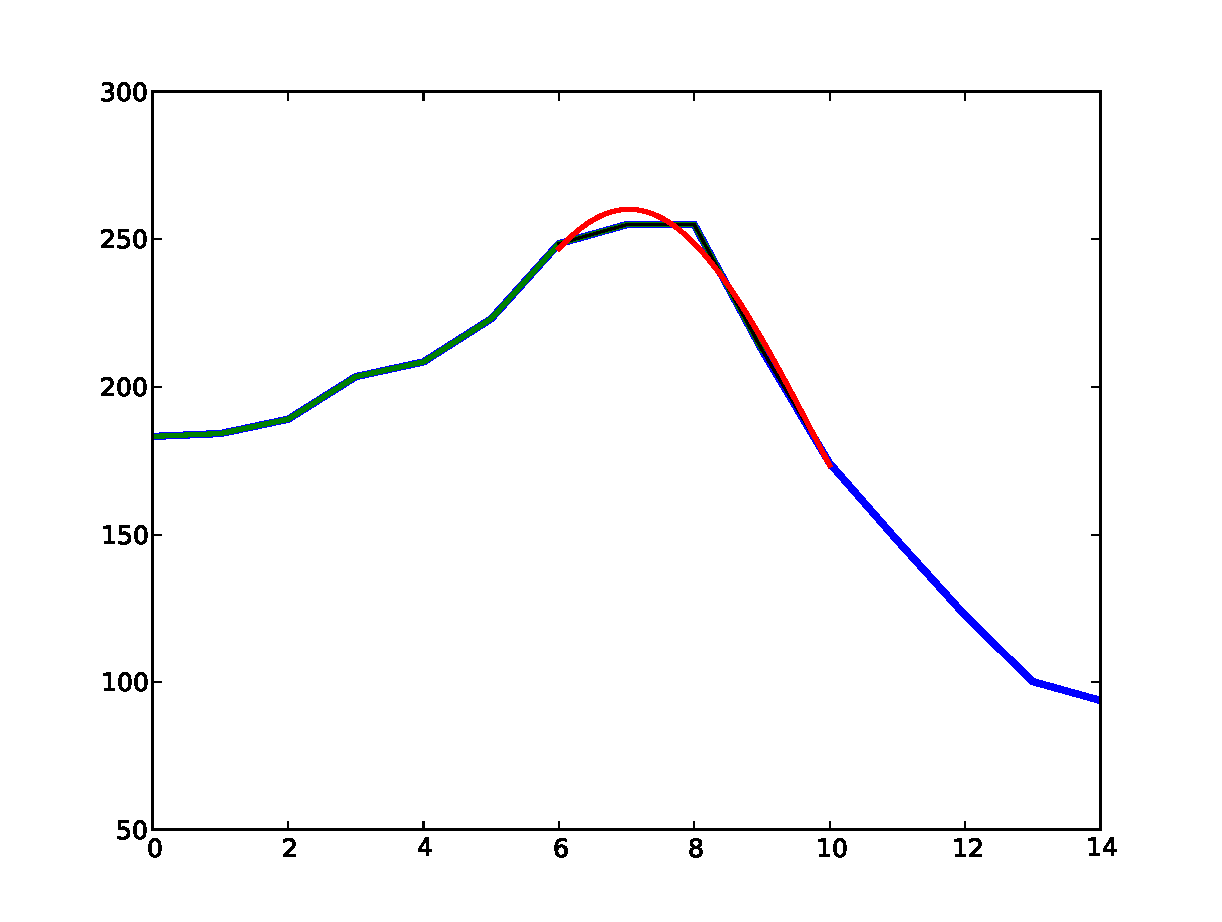
\includegraphics[width=\columnwidth]{figs/fitpeak.pdf}%
\caption{Fitting the peak with the Gauss profile. Blue + Green + Black - initial profile. After that the peak is shortened (Green + Black parts), then only symmetric part (Black) is considered for fitting (Red).}%
\label{fig:fitpeak}%
\end{figure}

\subsubsection{Fitting jumps}\label{fitjump}
Only the estimated position of the feature is provided to fitting routine together with the whole profile. Then routine finds the direction of the jump and searches for nearest local minimum and maximum. Then the resulting range plus-minus one data point is fitted with suitable function, which,  according to \cite{Bitler1999}, for brightness jumps in phase contrast images was chosen to be integral sine (\verb|scipy.special.sici()[0]|) (see Fig.~\ref{fig:fitedge}).

\begin{figure}%
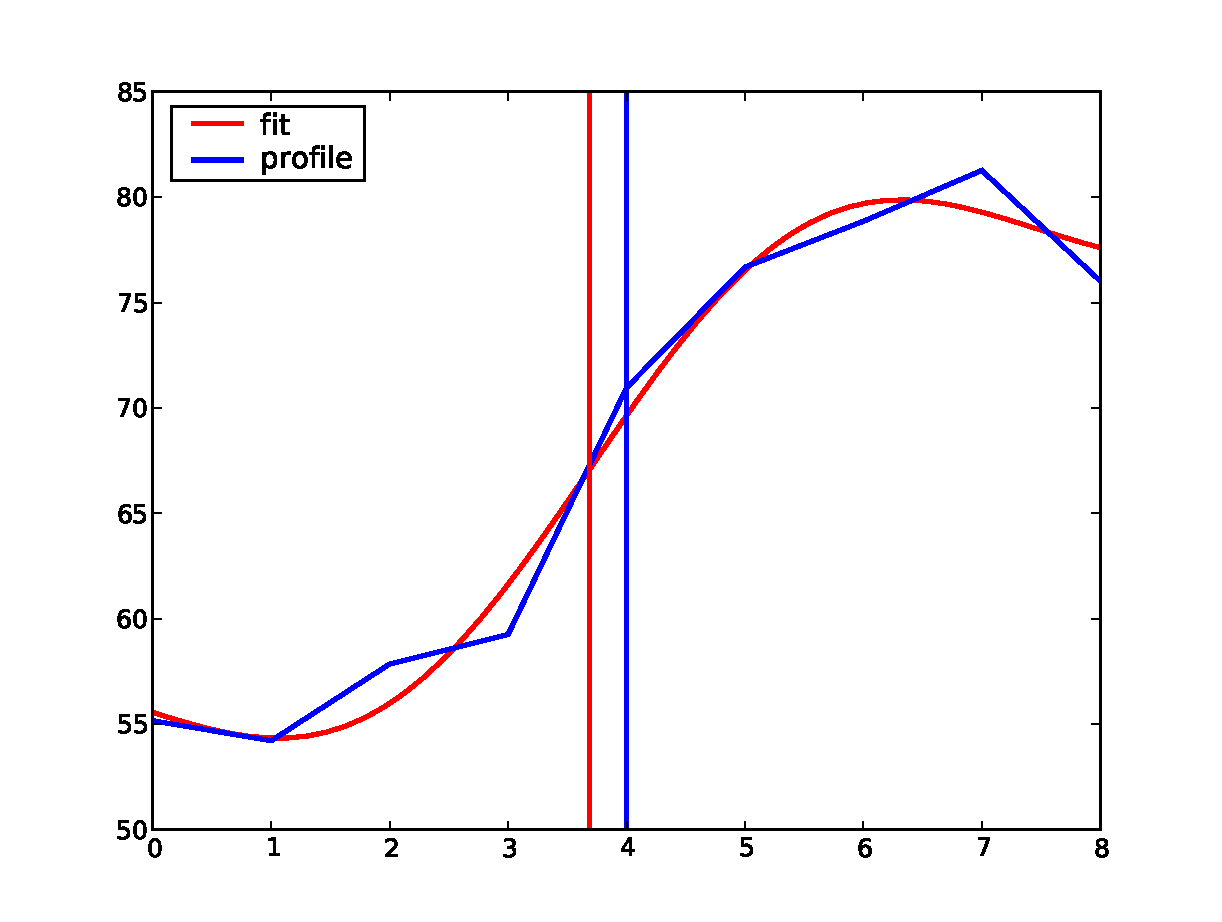
\includegraphics[width=\columnwidth]{figs/fitedge.pdf}%
\caption{Fitting the jump in brightness with integral sine. Blue - initial profile with position of the feature. Red - result of fitting and new feature position with subpixel resolution.}%
\label{fig:fitedge}%
\end{figure}

\subsection{Calculation of derived parameters}\label{results}

\begin{figure}%
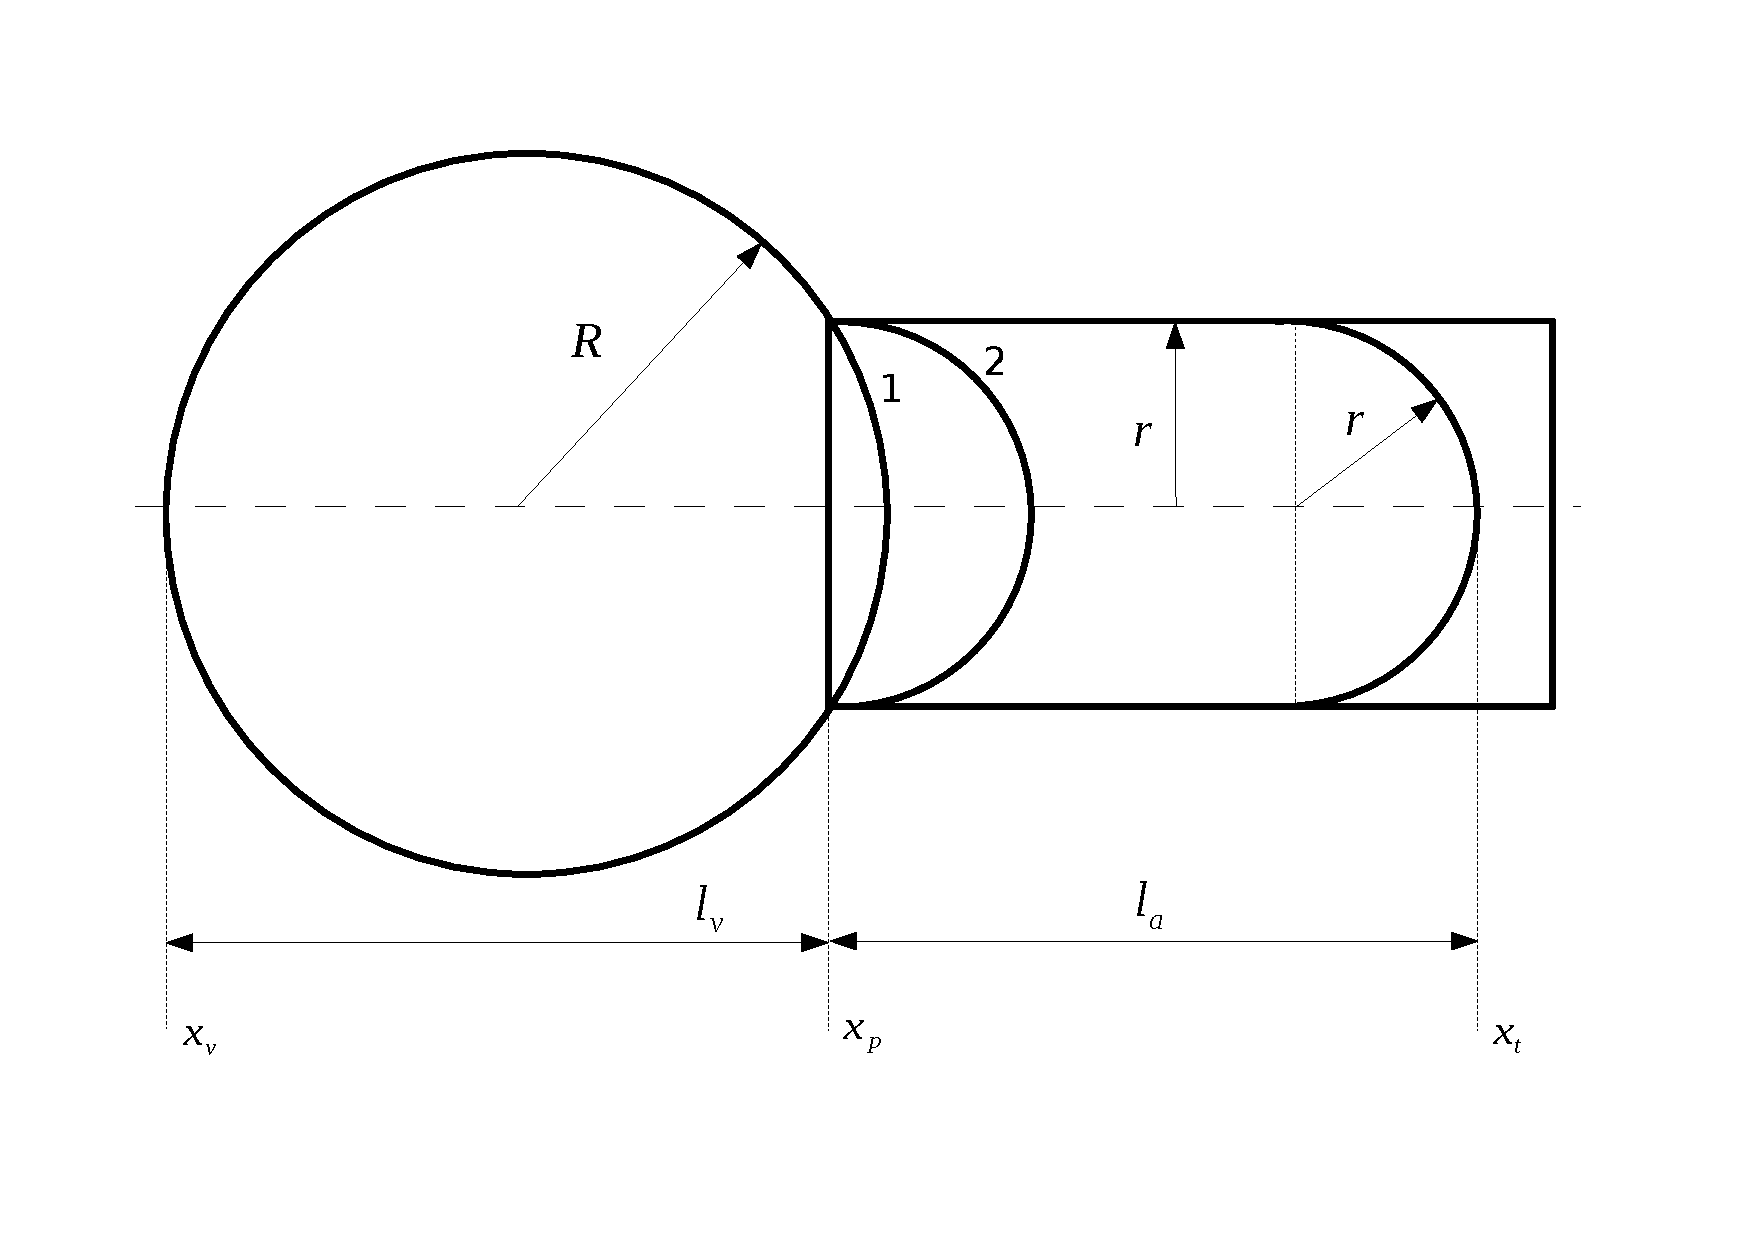
\includegraphics[width=\columnwidth]{figs/pipettesketch.pdf}%
\caption{Sketch of a vesicle aspirated into the pipette with explanation of parameters.\newline1: $l_a = 2R-l_v$.\newline2: $l_a = r$}%
\label{fig:pipettesketch}%
\end{figure}

Given positions of outer vesicle edge as $x_v$, pipette tip $x_p$ and aspirated vesicle tip $x_t$ plus the pipette radius $r$ together with their corresponding errors $\delta x_v$, $\delta x_p$, $\delta x_t$ and $\delta r$ and assuming total cylindrical symmetry of the system along the system axis and spherical form of the vesicle outside the pipette one can calculate the desired parameters (see Fig.~\ref{fig:pipettesketch}).

Denoting length of the vesicle part outside the pipette as $l_v = \left|x_p-x_v\right|$ with error $\delta l_v = \delta x_p + \delta x_v$ and the length of the aspirated tip as $l_a = \left|x_p-x_t\right|$ with error $\delta l_a = \delta x_p + \delta x_t$, the radius of the outside vesicle is
\begin{equation*}
R = \frac{{l_v}^2 + r^2}{2l_v}\;\;.
\end{equation*}
Corresponding error is then
\begin{equation*}
 \delta R = \sqrt{\frac{r^2}{{l_v}^2} \left(\delta r\right)^2 + \frac{1}{4}\left(1-\frac{r^2}{{l_v}^2}\right)^2 \left( \delta l_v\right) ^2}\;\;.
\end{equation*}
The surface of the inner part is
\begin{equation*}
S_\text{in} = \left\{
\begin{array}{ll}
	2\pi rl_a,& \text{if } l_a \geq r\\
	\pi\left({l_a}^2+r^2\right),&\text{if } 2R-l_v \leq l_a < r
\end{array}
\right.\;\;,
\end{equation*}
and its volume is
\begin{equation*}
V_{\text{in}} = \left\{
\begin{array}{ll}
	\pi r^2\left(l_a-\frac{r}{3}\right), & \text{if } l_a \geq r\\
	\frac{1}{6}\pi l_a\left(3r^2+{l_a}^2\right),&\text{if } 2R-l_v \leq l_a < r
\end{array}
\right.\;\;,
\end{equation*}
with errors
\begin{equation*}
 \delta S_\text{in} = \left\{
 \begin{array}{ll}
	2\pi \sqrt{{l_a}^2\left(\delta r\right)^2 + r^2\left(\delta l_a\right)^2},& \text{if } l_a \geq r\\
	2\pi \sqrt{{l_a}^2\left(\delta l_a\right)^2 + r^2\left(\delta r\right)^2},&\text{if } 2R-l_v \leq l_a < r
\end{array}
\right.\;\;
\end{equation*}
and
\begin{equation*}
\delta V_{\text{in}} = \left\{
\begin{array}{ll}
	\pi r \sqrt{r^2\left(\delta l_a\right)^2 + \left(2l_a-r\right)^2 \left(\delta r\right)^2}, & \text{if } l_a \geq r\\
	\frac{\pi}{2} \sqrt{4 r^2 {l_a}^2\left(\delta r\right)^2 + \left(r^2+{l_a}^2\right)^2 \left(\delta l_a\right)^2}, & \text{if } 2R-l_v \leq l_a < r
\end{array}
\right.\;\;.
\end{equation*}
The surface of the outer vesicle part is
\begin{equation*}
S_\text{out} = 2\pi Rl_v = \pi \left({l_v}^2+r^2\right)\;\;,
\end{equation*}
and it's volume is
\begin{equation*}
V_\text{out} = \frac{1}{6}\pi l_v\left(3r^2+{l_v}^2\right)\;\;
\end{equation*}
with errors
\begin{equation*}
\delta S_\text{out} = 2\pi\sqrt{{l_v}^2 \left(\delta l_v\right)^2 + r^2 \left( \delta r\right) ^2}\;\;
\end{equation*}
and
\begin{equation*}
\delta V_\text{out} = \frac{\pi}{2} \sqrt{4 r^2 {l_v}^2\left(\delta r\right)^2 + \left(r^2+{l_v}^2\right)^2 \left(\delta l_v\right)^2}\;\;.
\end{equation*}
Total area and volume of the vesicle are then $S = S_\text{out}+S_\text{in}$ and $V = V_\text{out}+V_\text{in}$ with errors $\delta S = \delta S_\text{out} + \delta S_\text{in}$ and $\delta V = \delta V_\text{out} + \delta V_\text{in}$ respectively.

\section{Data Analysis}\label{analysis}
\subsection{Classical procedure}
Having combined data acquired from image analysis together with corresponding pressure values obtained in experiment one finds elastic properties of membrane by fitting low-tension regime with logarithm and high-tension regime with linear functions. Also some corrections pointed out in \cite{Henriksen2004, Fournier2001} could be accounted for here, by trying to fit the whole range of pressures with one general function.

Currently tensions are calculated according to simple model after Evans:
\begin{equation}
\tau = \frac{P R_p}{2\left(1-\frac{R_p}{R_v}\right)}
\label{eq:tau-evans}
\end{equation}

Below is the list of currently implemented models/fittings.

Dilations:
\begin{itemize}
	\item simplest model $\alpha = \frac{S-S_0}{S_0}$
	\item corrected for initial aspiration after \cite{Henriksen2004}
	\begin{equation}
		\alpha = \left[
		 \frac{1}{2} \left(\frac{R_p}{R_{v0}}\right)^2 \frac{\Delta L}{R_p} 
		 + \left[1-\frac{3}{4}\left(\frac{R_p}{R_{v0}}\right)^3 \frac{\Delta L}{R_p} \right]^{\frac{2}{3}}
		 - 1 
		\right]\gamma
		\label{eq:alpha-henriksen}
	\end{equation}
	where $\displaystyle{\gamma = 1-\frac{2R_p L_0+R_p^2}{4R_{v0}^2}}$.
\end{itemize}

Fittings (done with Orthogonal Distance Regression):
\begin{itemize}
	\item Simple model for bending rigidity: $\alpha=\frac{1}{8\pi\kappa}\ln{\frac{\tau}{\tau_0}}$
	\item Simple model for stretching elasticity: $\alpha=\frac{\tau}{K}+\alpha_0$
\end{itemize}

\subsection{Modern procedure}
The overall ultimate goal is to implement a MCMC (Markov Chain Monte Carlo) algorithm found in  \cite{Henriksen2004}.